\section{Planering och genomförande}
% TODO: Kort och orienterande om hur ni tänkte genomföra uppgiften.
%       Orienterande om Planering och Genomförande.

% ______________________________________________________________________________
\subsection{Planering}
% Hur kommer ni att arbeta?  Detta är en lite längre text än den rent
% orienterande texten i Planering och genomförande ovan.  För att infoga
% hänvisningar till andra delar av dokumentet hittar ni under menyn
% ”Infoga/Korshänvisning...”.  Där kan ni skapa referenser som ni kan använda
% och ni kan lägga in sidnummer, kapitelnummer eller kapiteltext till en rubrik
% eller referens.

\begin{itemize}
  \item Laborationen utförs på en \texttt{ProBook-6545b} laptop som kör
        \texttt{Xubuntu 15.10} på \texttt{Linux 3.19.0-28-generic}.

  \item Rapporten skrivs i \LaTeX\ med texteditorn \texttt{Vim} och kompileras
        till pdf med \texttt{latexmk}.

  \item För revisionskontroll används \texttt{Git}.

  \item Virtualisering sker med \texttt{VirtualBox} version
        \texttt{5.0.10\_Ubuntu r104061}.

\end{itemize}

% ______________________________________________________________________________
\subsection{Genomförande}
Det första steget var att ladda hem en bootbar \texttt{.iso}-fil av
distributionen Debian. Det finns många olika varianter att välja bland och då
jag sedan tidigare är van vid att använda \texttt{xfce} så valde jag att ladda
hem \texttt{debian-live-8.2.0-i386-xfce-desktop} som är en variant av Debian
som levereras med den grafiska miljön \texttt{xfce}. Den Grafiska miljön är
bara en komponent av hela systemet som lätt kan bytas ut vid ett senare
tillfälle, så att välja precis ``rätt'' paktererad version av en distribution
är inte nödvändigt.  Men en färdigpaketerad version brukar kunna förenkla
installationsprocessen.

\begin{figure}[htbp]
  \centering
    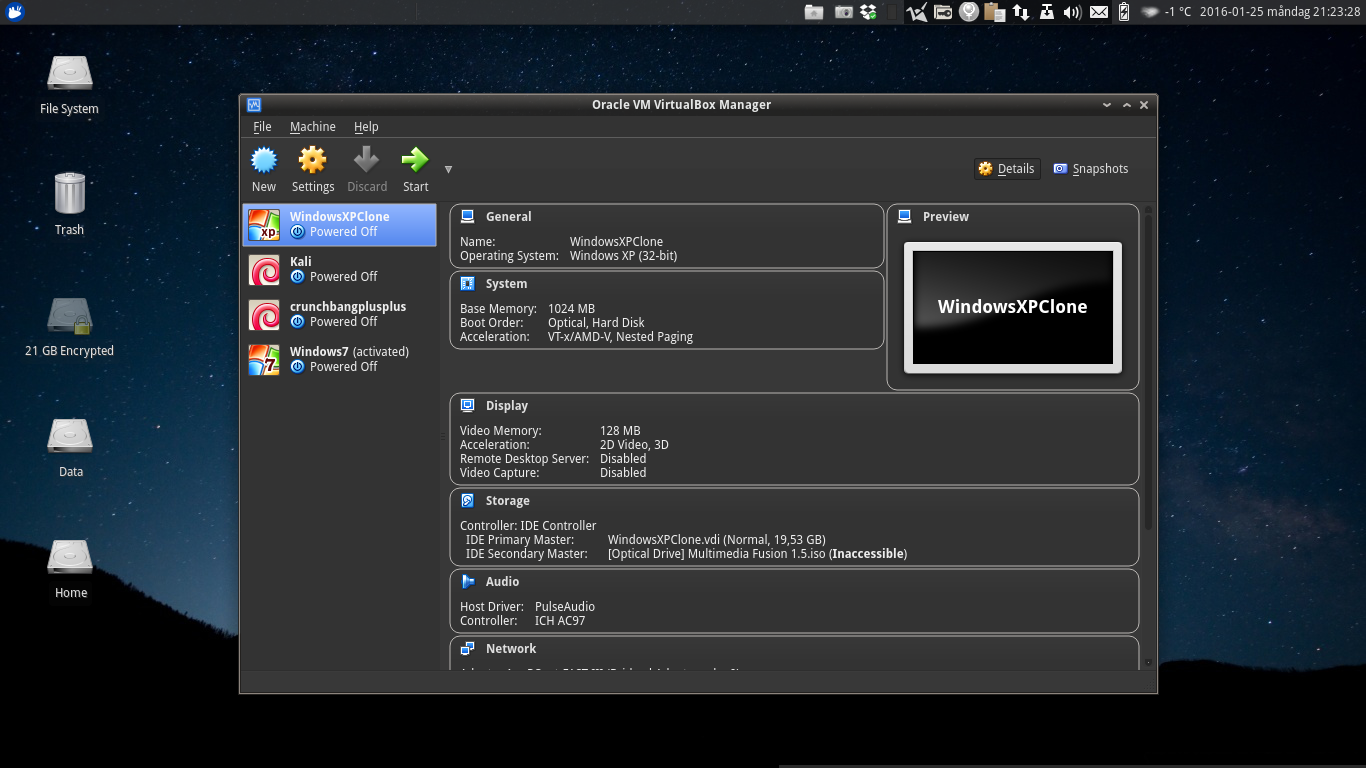
\includegraphics[width=\linewidth]{img/A_new-01}
    \caption{Skärmdump av värdsystemet som kör \texttt{VirtualBox} där en ny
             virtuell maskin skapas genom att klicka den blå ikonen \texttt{New}.}
  \label{fig:A_new-01}
\end{figure}

Jag väljer att skapa min miljö som en virtuell maskin. Då jag redan använder
och är bekant med \texttt{VirtualBox} så väljer jag att använda det för att
skapa min virtuella maskin enligt Figur~\ref{fig:A_new-01}.

% Här skriver ni vilka steg ni gjorde och resultatet av dem. Ni skall ha med
% information så att vi kan se hur ni har gjort, dvs beskrivande text,
% skärmdumpar, bilder etc.  Längre skärmdumpar, innehåll i relevanta filer och
% större bilder lägger ni i bilagor, som bilaga I, så att de inte tar över en
% sida själva.
% Kommandon som ni skriver i ett skal skall skrivas i detta format, som är
% teckenformatmall ”Exempel” i OpenOffice/LibreOffice. Detta så att de
% skiljer sig från övriga brödtext i stycket.  Detta underlättar läsningen för
% andra, som oss lärare.
% Bilder lägger ni in med "Infoga/Bildobjekt/Från fil..." och sedan lägger ni
% till text och numrering genom att markera bilden och sedan göra
% "Infoga/Bildtext...".  Notera att man har det finns olika bildtext för dem
% som vill prova. I den här har jag valt illustration samt skrivit in en liten
% förklarande text.  Till bilden kan man sedan infoga en referens där man anger
% Illustration och sedan väljer önskad bild.


\begin{figure}[htbp]
  \centering
  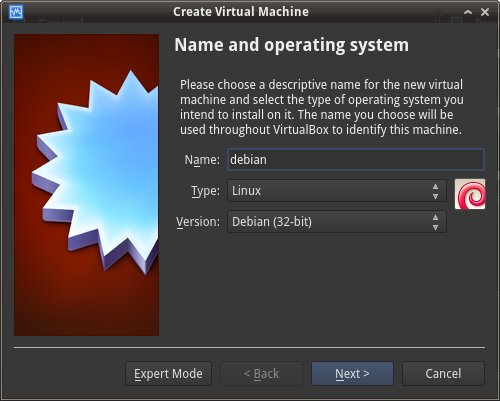
\includegraphics[width=0.7\linewidth]{img/A_new-02}
  \caption{I dialogrutan för en ny virtuell maskin väljs namnet
           \texttt{debian}. Autodetektering baserat på det inmatade
           namnet markerar automatiskt \texttt{Type} samt \texttt{Version}
           som i det här fallet stämmer och är lämpliga inställningar.}
  \label{fig:A_new-02}
\end{figure}

\begin{figure}[htbp]
  \centering
  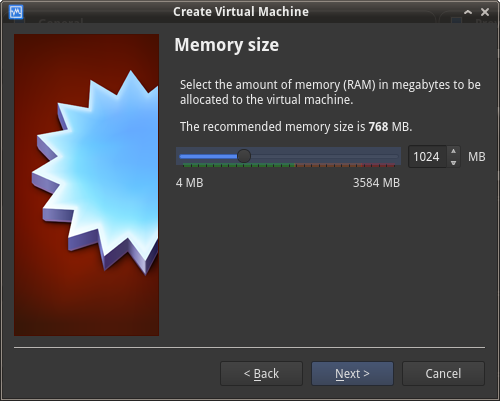
\includegraphics[width=\linewidth]{img/A_new-03}
  \caption{Storleken på RAM-minnet sätts till en lämplig kompromiss mellan
           vad värdsystemet kan tänkas behöva och vad gästsystemet kräver.}
  \label{}
\end{figure}

\begin{figure}[htbp]
  \centering
  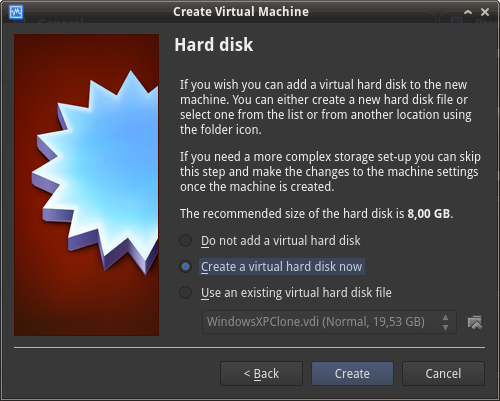
\includegraphics[width=\linewidth]{img/A_new-04}
  \caption{I dialogrutan för hårddisk väljer vi att skapa en ny virtuell
           hårddisk.}
  \label{}
\end{figure}

\begin{figure}[htbp]
  \centering
  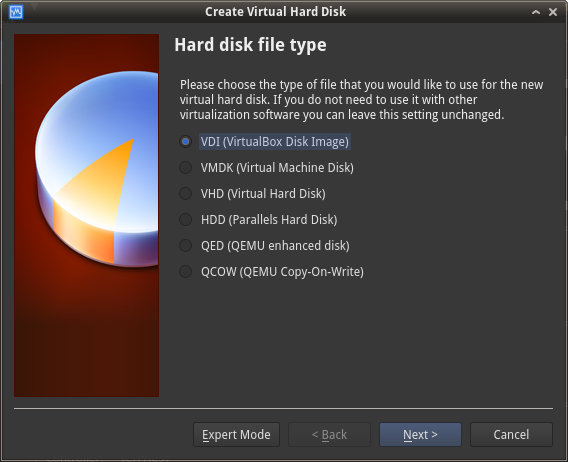
\includegraphics[width=\linewidth]{img/A_new-05}
  \caption{Standardvalet \texttt{VDI} fungerar bra för det här
           användningsområdet. Ytterigare information de olika alternativen
           finns i \cite{virtualbox:vdidetails}.}
           % TODO: FIXA OVANSTÅENDE!
  \label{}
\end{figure}

\begin{figure}[htbp]
  \centering
  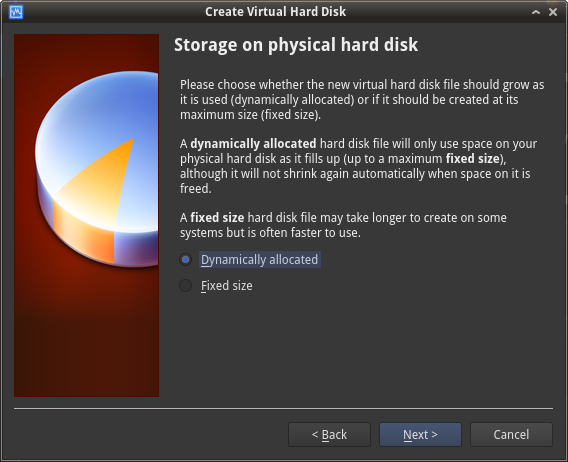
\includegraphics[width=\linewidth]{img/A_new-06}
  \caption{Lagringsutrymmets storlek väljs att växa dynamiskt efter behov.}
  \label{}
\end{figure}

\begin{figure}[htbp]
  \centering
  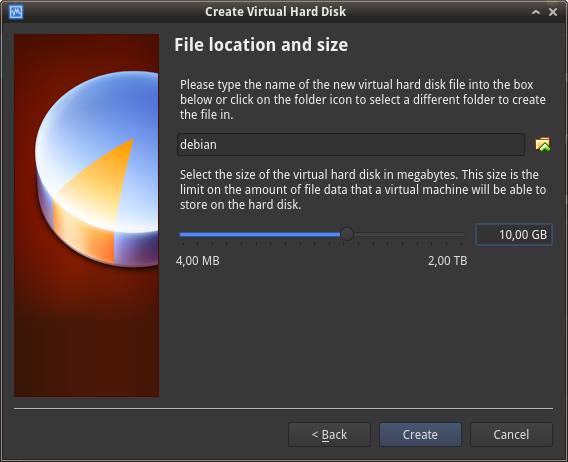
\includegraphics[width=\linewidth]{img/A_new-07}
  \caption{Namnet och storleken på disken sätts till \texttt{debian} (vilket
           ger ett filnamn \texttt{debian.vdi} i katalogen för den virtuella
           maskinen) och storleken sätts godtyckligt till \SI{10}{\mebi\byte}.}
  \label{}
\end{figure}

\screenshot{img/A_new-08}
           {Ytterligare inställningsmöjligheter kan göras genom att högerklicka
            på den virtuella maskinen vi skapat och välja \texttt{Settings}.}
           {labell}
